\chapter{Chapter 2}
\chaptermark{Chapter 2}
\label{ch:chapter02}

\noindent\textbf{ECC-DTB-AKA: Device- and Transaction-Bound Authenticated Key Agreement for Client-Server E-Banking Channels}\par

\section{Introduction and Motivation}\indent Chapter 1 identified six critical limitations in current authentication and key-exchange mechanisms deployed in e-banking client-server channels (Section 1.2.3). These limitations---decoupled transport and application authentication, absence of device binding, lack of per-transaction key derivation, bearer-token vulnerability, insufficient message-level integrity across service boundaries, and legacy TLS configurations without forward secrecy---collectively create exploitable gaps that attackers leverage through session hijacking, credential replay, and man-in-the-middle attacks.

\indent This chapter proposes ECC-DTB-AKA (Elliptic Curve Cryptography --- Device- and Transaction-Bound Authenticated Key Agreement), an alternative approach to strengthening security systems in e-banking and e-finance environments. ECC-DTB-AKA integrates mutual authentication, ephemeral ECDH key agreement, device fingerprint binding, and on-demand transaction key derivation into a unified three-round protocol. By incorporating device and transaction context directly into the HKDF key-derivation salt, the scheme ensures that session keys and transaction keys are cryptographically bound to the originating device and specific financial operation, addressing limitations that existing TLS-centric and OAuth-based approaches cannot resolve without additional protocol layers.

\indent The design philosophy of ECC-DTB-AKA follows the principle of cryptographic cohesion: rather than stacking independent security layers (TLS for transport, JWT for session, OTP for transaction), all authentication and key-establishment functions are unified within a single ECC-based protocol. This reduces the attack surface at layer boundaries and provides formal security properties that can be analyzed within a single proof framework.

\subsection{Limitations of Layered Security Architectures}\indent Contemporary e-banking systems typically implement security as a vertical stack of independent layers: network firewalls at the perimeter, TLS at the transport layer, web application firewalls at the HTTP layer, authentication middleware at the application layer, and database encryption at the persistence layer. While defense-in-depth is a sound principle, the interfaces between layers create implicit trust assumptions that attackers exploit.

\indent Consider a typical mobile banking login flow: (1) the mobile app establishes a TLS 1.3 connection to the API gateway, authenticating the server via its certificate; (2) the user enters credentials, which the app transmits over the TLS channel; (3) the authentication service validates credentials and returns a JWT session token; (4) subsequent API calls include the JWT in the Authorization header, still over TLS. At each layer boundary, data transitions between protection domains. The TLS layer knows nothing about the user's identity; the JWT layer knows nothing about the encryption keys; the transaction layer knows nothing about the originating device.

\indent An attacker who compromises the JWT (via malware, XSS, or network interception on a misconfigured endpoint) gains full session access without breaking TLS. An attacker who performs SSL stripping at a captive portal downgrades the transport layer while the application layer continues to function, potentially exposing credentials. ECC-DTB-AKA collapses layers 1--3 into a single cryptographic protocol where user identity, device context, and session keys are established atomically.

\section{Design Goals and Requirements}\indent Derived from the security requirements SR1--SR4 and SR8 established in Section 1.4.5, ECC-DTB-AKA is designed to satisfy the following goals:

\indent G1 (Mutual Authentication): Both client and server must cryptographically prove their identity during key establishment, not merely after an encrypted channel is created.

\indent G2 (Forward Secrecy): Compromise of long-term private keys must not enable retroactive decryption of previously established sessions.

\indent G3 (Device Binding): Session keys must incorporate a device fingerprint in the derivation function, preventing session transfer to unauthorized devices.

\indent G4 (Transaction Binding): Per-transaction keys must be derivable from the session master key without additional communication rounds.

\indent G5 (Efficiency): Authentication must complete with minimal latency and message overhead, suitable for mobile banking on cellular networks.

\indent G6 (Standards Alignment): The protocol must use NIST-approved curves (SECP256R1), SHA-256, HKDF (RFC 5869), and ECDSA (FIPS 186-5), enabling integration with existing PKI and HSM infrastructure.

\subsection{Elliptic Curve Cryptography Foundations}\indent The selection of elliptic curve cryptography as the sole public-key primitive in ECC-DTB-AKA warrants explicit justification given the availability of alternatives (RSA, DSA, post-quantum algorithms).

\indent Elliptic curves over finite fields provide a group structure in which the Diffie-Hellman problem is hard: given G, [a]G, [b]G, computing [ab]G is computationally infeasible. The security level of SECP256R1 (NIST P-256) is approximately 128 bits, equivalent to AES-128 and SHA-256. The key size of 256 bits compares favorably to 3072-bit RSA keys for equivalent security, reducing bandwidth, storage, and computation.

\indent SECP256R1 is specified in FIPS 186-5 and SP 800-186, widely implemented in hardware (HSMs, smart cards, TPMs), and supported by every major TLS library. Its curve parameters were generated verifiably (though debates about potential backdoors in NIST curves persist in the literature; Curve25519 is an alternative that ECC-DTB-AKA could adopt with minimal protocol changes). For e-banking deployments requiring FIPS compliance, SECP256R1 is the pragmatic choice.

\indent ECDSA signatures on SECP256R1 provide the authentication mechanism in ECC-DTB-AKA. Each signature operation requires one scalar multiplication and one modular inversion, typically completing in under 1 ms on modern processors. The prototype measurements confirm that four signature operations per handshake (two per party) dominate the computational cost, accounting for approximately 80\% of total authentication latency.

\section{Protocol Specification}\indent This section provides the complete specification of ECC-DTB-AKA, including notation, algorithmic descriptions, and message formats. The protocol operates between a banking client C and banking server S over an insecure channel.

\subsection{Notation and Prerequisites}\indent Let E/ F\textbackslash\{\}textsubscript\{p\} be the elliptic curve SECP256R1 with generator G and prime order q. H: \{0,1\}* → \{0,1\}\textasciicircum{}256 denotes SHA-256. HKDF\textbackslash\{\}textsubscript\{extract\} and HKDF\textbackslash\{\}textsubscript\{expand\} denote the extract and expand functions per RFC 5869. || denotes concatenation. C holds a long-term key pair (sk\textbackslash\{\}textsubscript\{C\}, PK\textbackslash\{\}textsubscript\{C\} = [sk\textbackslash\{\}textsubscript\{C\}]G) registered with S during account enrollment. S holds a long-term key pair (sk\textbackslash\{\}textsubscript\{S\}, PK\textbackslash\{\}textsubscript\{S\} = [sk\textbackslash\{\}textsubscript\{S\}]G) with an X.509 certificate issued by the bank's CA. device\textbackslash\{\}textsubscript\{fp\} = H(hardware\textbackslash\{\}textsubscript\{attributes\})_\{128\} is a 128-bit device fingerprint computed from stable hardware attributes (platform ID, secure enclave identifier). Each protocol run generates ephemeral key pairs (ek\textbackslash\{\}textsubscript\{C\}, EK\textbackslash\{\}textsubscript\{C\} = [ek\textbackslash\{\}textsubscript\{C\}]G) and (ek\textbackslash\{\}textsubscript\{S\}, EK\textbackslash\{\}textsubscript\{S\} = [ek\textbackslash\{\}textsubscript\{S\}]G).

\subsection{Round 1 --- Client Init (MSG1)}\indent The client initiates the protocol by generating an ephemeral key pair (ek\textbackslash\{\}textsubscript\{C\}, EK\textbackslash\{\}textsubscript\{C\}), sampling a 128-bit nonce nonce\textbackslash\{\}textsubscript\{c\} ← \{0,1\}\textasciicircum{}128, and computing the transcript hash t\textbackslash\{\}textsubscript\{C\} = H(EK\textbackslash\{\}textsubscript\{C\} || PK\textbackslash\{\}textsubscript\{C\} || device\textbackslash\{\}textsubscript\{fp\} || nonce\textbackslash\{\}textsubscript\{c\}). The client signs this hash with its long-term private key: σ_C = Sig_\{sk\textbackslash\{\}textsubscript\{C\}\}(t\textbackslash\{\}textsubscript\{C\}). The first message is MSG1 = (EK\textbackslash\{\}textsubscript\{C\}, PK\textbackslash\{\}textsubscript\{C\}, device\textbackslash\{\}textsubscript\{fp\}, nonce\textbackslash\{\}textsubscript\{c\}, σ_C).

\indent MSG1 serves three purposes: (1) the ephemeral public key EK\textbackslash\{\}textsubscript\{C\} enables ECDH key agreement; (2) the long-term public key PK\textbackslash\{\}textsubscript\{C\} and signature σ_C authenticate the client; (3) the device fingerprint and nonce bind the session to a specific device and prevent replay of prior MSG1 values.

\begin{figure}[htbp]
\centering
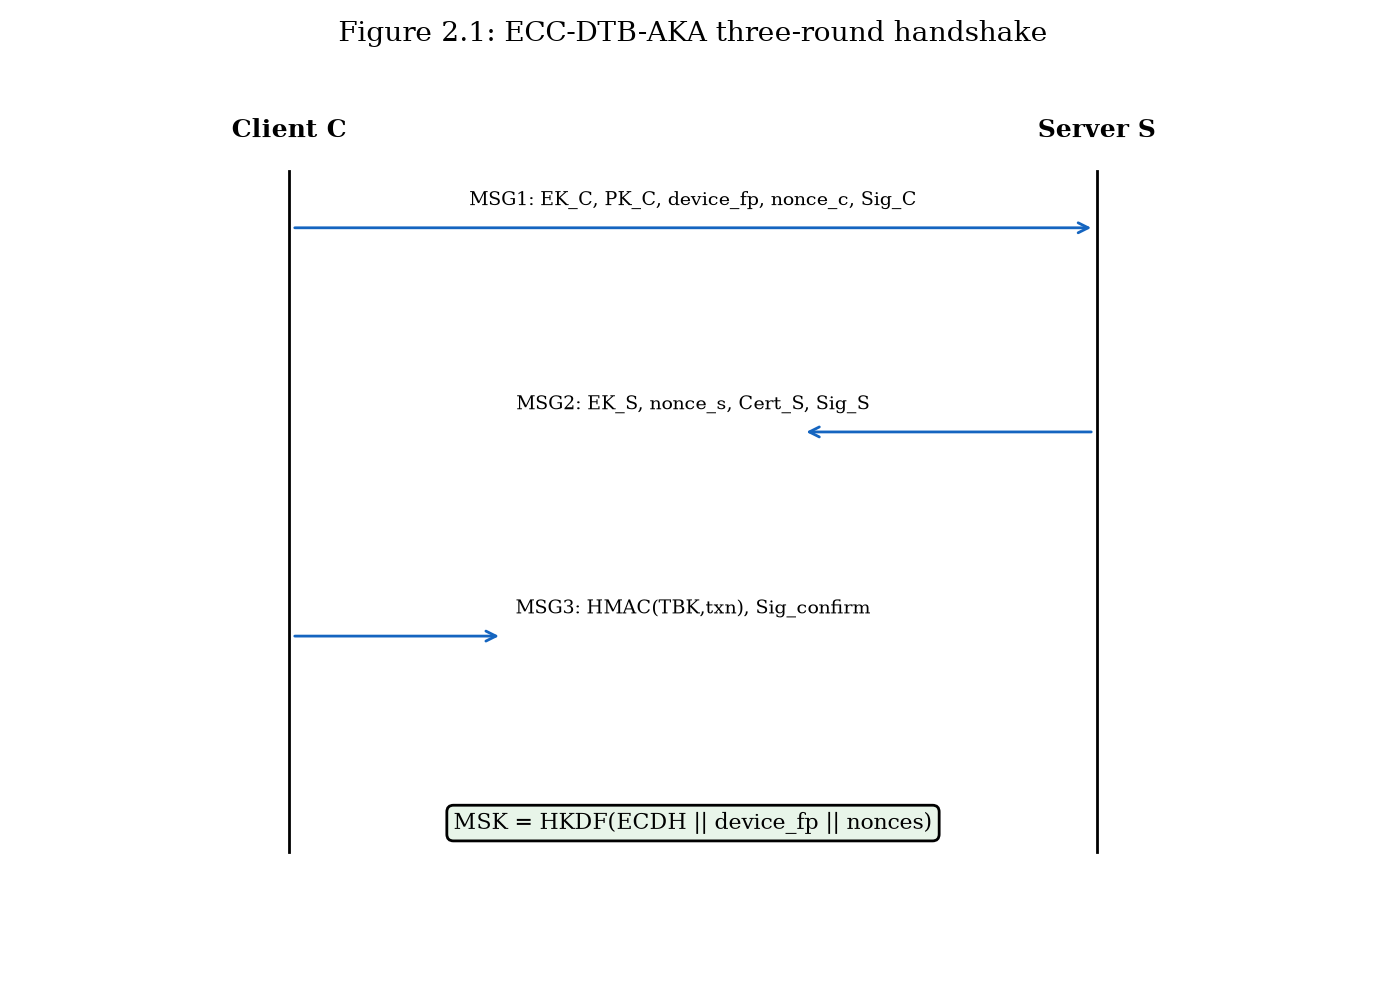
\includegraphics[width=0.92\linewidth]{../thesis/figures/fig_2_1_protocol_sequence.png}
\caption{ECC-DTB-AKA three-round handshake sequence diagram (Figure 2.1).}
\end{figure}

\subsection{Round 2 --- Server Response (MSG2)}\indent Upon receiving MSG1, the server performs the following steps: (1) Look up PK\textbackslash\{\}textsubscript\{C\} in the customer registry; reject if not found. (2) Verify σ_C against t\textbackslash\{\}textsubscript\{C\} using PK\textbackslash\{\}textsubscript\{C\}; reject if invalid. (3) Generate ephemeral (ek\textbackslash\{\}textsubscript\{S\}, EK\textbackslash\{\}textsubscript\{S\}) and sample nonce\textbackslash\{\}textsubscript\{s\} ← \{0,1\}\textasciicircum{}128. (4) Compute shared secret Z = [ek\textbackslash\{\}textsubscript\{S\}]EK\textbackslash\{\}textsubscript\{C\}. (5) Derive master session key MSK = HKDF(Z, device\textbackslash\{\}textsubscript\{fp\} || nonce\textbackslash\{\}textsubscript\{c\} || nonce\textbackslash\{\}textsubscript\{s\}, 'ECC-DTB-AKA-v1', 256). (6) Compute σ_S = Sig_\{sk\textbackslash\{\}textsubscript\{S\}\}(H(EK\textbackslash\{\}textsubscript\{S\} || nonce\textbackslash\{\}textsubscript\{s\} || MSK)). (7) Send MSG2 = (EK\textbackslash\{\}textsubscript\{S\}, nonce\textbackslash\{\}textsubscript\{s\}, Cert\textbackslash\{\}textsubscript\{S\}, σ_S).

\indent The server signature over EK\textbackslash\{\}textsubscript\{S\}, nonce\textbackslash\{\}textsubscript\{s\}, and MSK provides key confirmation: the client can verify that the server computed the same MSK before proceeding. The server certificate Cert\textbackslash\{\}textsubscript\{S\} enables the client to validate server identity through the bank's PKI chain.

\subsection{Round 3 --- Client Confirm (MSG3)}\indent The client verifies Cert\textbackslash\{\}textsubscript\{S\}, recomputes Z = [ek\textbackslash\{\}textsubscript\{C\}]EK\textbackslash\{\}textsubscript\{S\} and MSK, and validates σ_S. For a pending transaction with nonce txn\textbackslash\{\}textsubscript\{nonce\}, the client derives the transaction-bound key TBK\textbackslash\{\}textsubscript\{txn\} = HKDF(MSK, txn\textbackslash\{\}textsubscript\{nonce\}, 'TBK', 256) and computes τ = HMAC(TBK\textbackslash\{\}textsubscript\{txn\}, txn\textbackslash\{\}textsubscript\{nonce\}). The client sends MSG3 = (τ, txn\textbackslash\{\}textsubscript\{nonce\}, Sig_\{sk\textbackslash\{\}textsubscript\{C\}\}(H(MSK || 'confirm'))).

\indent The server verifies the client confirmation signature, recomputes TBK\textbackslash\{\}textsubscript\{txn\}, and validates τ. Upon success, both parties hold MSK and can derive additional transaction keys for subsequent operations without further handshakes until session expiration.

\begin{figure}[htbp]
\centering
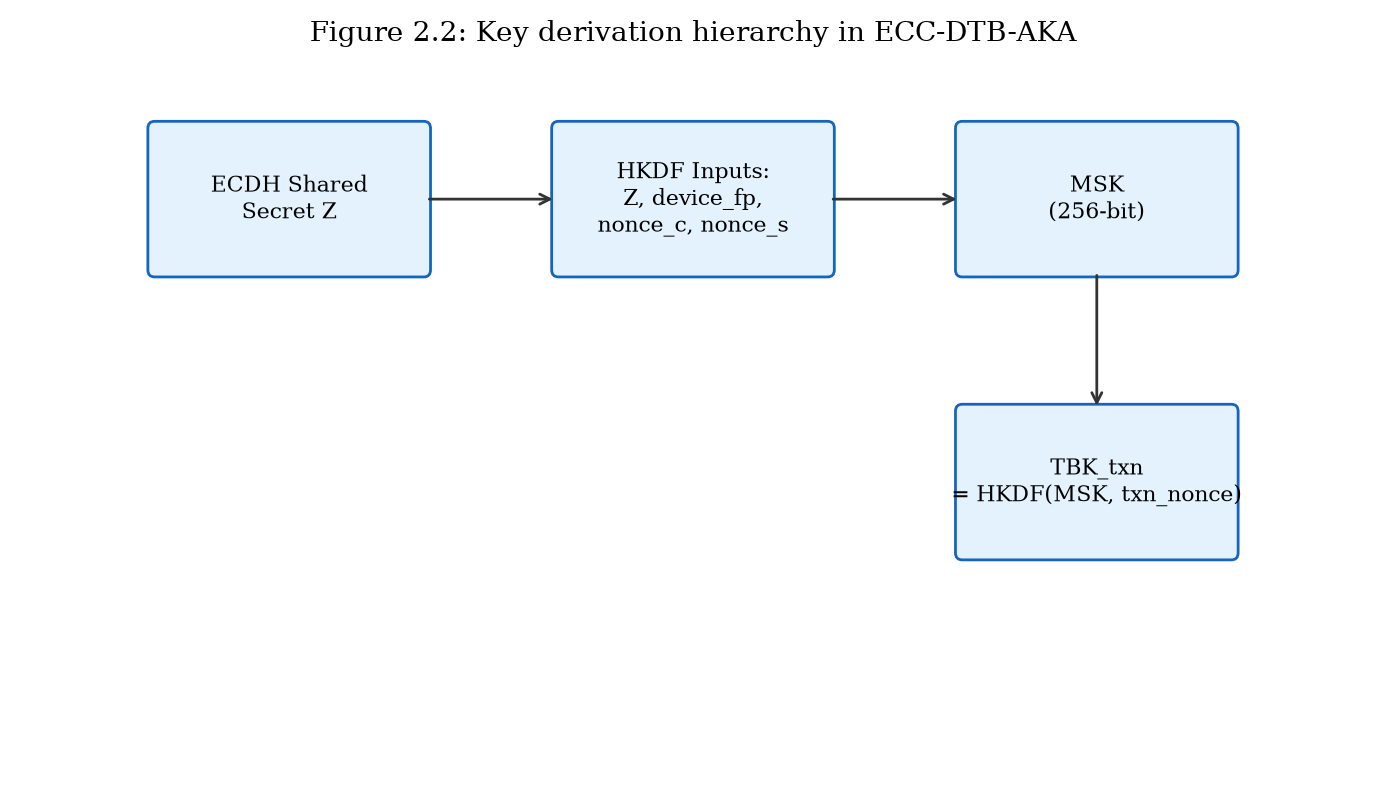
\includegraphics[width=0.92\linewidth]{../thesis/figures/fig_2_2_key_derivation.png}
\caption{Key derivation hierarchy from ECDH shared secret to MSK and TBK\textbackslash\{\}textsubscript\{txn\} (Figure 2.2).}
\end{figure}

\subsection{Transaction Key Derivation}\indent A distinguishing feature of ECC-DTB-AKA is the ability to derive per-transaction keys from the established MSK without additional protocol rounds. For each transaction T\textbackslash\{\}textsubscript\{i\} with unique nonce txn\textbackslash\{\}textsubscript\{nonce\}_i, both parties compute TBK\textbackslash\{\}textsubscript\{i\} = HKDF(MSK, txn\textbackslash\{\}textsubscript\{nonce\}_i, 'TBK', 256). Transaction data is protected using AES-256-GCM with TBK\textbackslash\{\}textsubscript\{i\} split into encryption and authentication subkeys. If a single transaction key is compromised, other transactions within the same session remain protected because HKDF derivation is one-way and domain-separated by distinct txn\textbackslash\{\}textsubscript\{nonce\} values.

\subsection{Message Format Summary}\indent Table 2.3 summarizes the wire-format fields for each protocol message. All integer fields are encoded in big-endian. Public keys use X9.62 uncompressed point format (65 bytes for P-256). Signatures are DER-encoded ECDSA (typically 70--72 bytes).

\indent The total payload for a complete handshake is approximately 569 bytes as measured in the prototype, making ECC-DTB-AKA suitable for bandwidth-constrained mobile networks. By comparison, a typical TLS 1.3 handshake with a 2 KB certificate chain exceeds 3 KB before application data.

\begin{table}[htbp]
\centering
\begin{tabular}{llll}
\toprule
Message & Field & Size (bytes) & Description \\
\midrule
MSG1 & EK\textbackslash\{\}textsubscript\{C\} & 65 & Client ephemeral public key \\
MSG1 & PK\textbackslash\{\}textsubscript\{C\} & 65 & Client long-term public key \\
MSG1 & device\textbackslash\{\}textsubscript\{fp\} & 16 & Device fingerprint \\
MSG1 & nonce\textbackslash\{\}textsubscript\{c\} & 16 & Client nonce \\
MSG1 & σ_C & \textasciitilde{}72 & ECDSA signature \\
MSG2 & EK\textbackslash\{\}textsubscript\{S\} & 65 & Server ephemeral public key \\
MSG2 & nonce\textbackslash\{\}textsubscript\{s\} & 16 & Server nonce \\
MSG2 & Cert\textbackslash\{\}textsubscript\{S\} & 65 & Server public key (prototype) \\
MSG2 & σ_S & \textasciitilde{}72 & ECDSA signature \\
MSG3 & τ & 32 & HMAC-SHA256 transaction tag \\
MSG3 & txn\textbackslash\{\}textsubscript\{nonce\} & 16 & Transaction nonce \\
MSG3 & σ_confirm & \textasciitilde{}72 & Client confirmation signature \\
\bottomrule
\end{tabular}
\caption{Table 2.3: ECC-DTB-AKA message field specification.}
\end{table}
\subsection{Algorithm: Client Handshake}\indent Algorithm 2.1 presents the client-side handshake procedure in pseudocode form. The algorithm takes as input the client's long-term key pair (sk\textbackslash\{\}textsubscript\{C\}, PK\textbackslash\{\}textsubscript\{C\}), device attributes, and an optional transaction nonce. It outputs the three protocol messages and the established session state.

\indent Algorithm 2.1 (ClientHandshake): (1) device\textbackslash\{\}textsubscript\{fp\} ← H(hardware\textbackslash\{\}textsubscript\{attributes\})[0:128]; (2) (ek\textbackslash\{\}textsubscript\{C\}, EK\textbackslash\{\}textsubscript\{C\}) ← KeyGen(E); (3) nonce\textbackslash\{\}textsubscript\{c\} ← \{0,1\}\textasciicircum{}128; (4) t\textbackslash\{\}textsubscript\{C\} ← H(EK\textbackslash\{\}textsubscript\{C\} || PK\textbackslash\{\}textsubscript\{C\} || device\textbackslash\{\}textsubscript\{fp\} || nonce\textbackslash\{\}textsubscript\{c\}); (5) σ_C ← ECDSA.Sign(sk\textbackslash\{\}textsubscript\{C\}, t\textbackslash\{\}textsubscript\{C\}); (6) MSG1 ← (EK\textbackslash\{\}textsubscript\{C\}, PK\textbackslash\{\}textsubscript\{C\}, device\textbackslash\{\}textsubscript\{fp\}, nonce\textbackslash\{\}textsubscript\{c\}, σ_C); Send(MSG1); (7) Receive(MSG2 = (EK\textbackslash\{\}textsubscript\{S\}, nonce\textbackslash\{\}textsubscript\{s\}, Cert\textbackslash\{\}textsubscript\{S\}, σ_S)); (8) Verify Cert\textbackslash\{\}textsubscript\{S\} against bank CA; (9) Z ← ECDH(ek\textbackslash\{\}textsubscript\{C\}, EK\textbackslash\{\}textsubscript\{S\}); (10) MSK ← HKDF(Z, device\textbackslash\{\}textsubscript\{fp\} || nonce\textbackslash\{\}textsubscript\{c\} || nonce\textbackslash\{\}textsubscript\{s\}, 'ECC-DTB-AKA-v1'); (11) Verify σ_S = ECDSA.Sign_\{PK\textbackslash\{\}textsubscript\{S\}\}(H(EK\textbackslash\{\}textsubscript\{S\} || nonce\textbackslash\{\}textsubscript\{s\} || MSK)); (12) TBK ← HKDF(MSK, txn\textbackslash\{\}textsubscript\{nonce\}, 'TBK'); (13) τ ← HMAC(TBK, txn\textbackslash\{\}textsubscript\{nonce\}); (14) MSG3 ← (τ, txn\textbackslash\{\}textsubscript\{nonce\}, ECDSA.Sign(sk\textbackslash\{\}textsubscript\{C\}, H(MSK || 'confirm'))); Send(MSG3); (15) Erase ek\textbackslash\{\}textsubscript\{C\}; Return (MSK, TBK).

\subsection{Algorithm: Server Handshake}\indent Algorithm 2.2 presents the server-side procedure. The server maintains a customer registry mapping PK\textbackslash\{\}textsubscript\{C\} to account metadata and validates each handshake against this registry.

\indent Algorithm 2.2 (ServerHandshake): (1) Receive(MSG1); (2) Look up PK\textbackslash\{\}textsubscript\{C\} in customer registry; abort if not found; (3) t\textbackslash\{\}textsubscript\{C\} ← H(EK\textbackslash\{\}textsubscript\{C\} || PK\textbackslash\{\}textsubscript\{C\} || device\textbackslash\{\}textsubscript\{fp\} || nonce\textbackslash\{\}textsubscript\{c\}); (4) Verify σ_C = ECDSA.Sign_\{PK\textbackslash\{\}textsubscript\{C\}\}(t\textbackslash\{\}textsubscript\{C\}); abort if invalid; (5) (ek\textbackslash\{\}textsubscript\{S\}, EK\textbackslash\{\}textsubscript\{S\}) ← KeyGen(E); (6) nonce\textbackslash\{\}textsubscript\{s\} ← \{0,1\}\textasciicircum{}128; (7) Z ← ECDH(ek\textbackslash\{\}textsubscript\{S\}, EK\textbackslash\{\}textsubscript\{C\}); (8) MSK ← HKDF(Z, device\textbackslash\{\}textsubscript\{fp\} || nonce\textbackslash\{\}textsubscript\{c\} || nonce\textbackslash\{\}textsubscript\{s\}, 'ECC-DTB-AKA-v1'); (9) σ_S ← ECDSA.Sign(sk\textbackslash\{\}textsubscript\{S\}, H(EK\textbackslash\{\}textsubscript\{S\} || nonce\textbackslash\{\}textsubscript\{s\} || MSK)); (10) MSG2 ← (EK\textbackslash\{\}textsubscript\{S\}, nonce\textbackslash\{\}textsubscript\{s\}, Cert\textbackslash\{\}textsubscript\{S\}, σ_S); Send(MSG2); (11) Receive(MSG3 = (τ, txn\textbackslash\{\}textsubscript\{nonce\}, σ_confirm)); (12) Verify σ_confirm = ECDSA.Sign_\{PK\textbackslash\{\}textsubscript\{C\}\}(H(MSK || 'confirm')); (13) TBK ← HKDF(MSK, txn\textbackslash\{\}textsubscript\{nonce\}, 'TBK'); (14) Verify τ = HMAC(TBK, txn\textbackslash\{\}textsubscript\{nonce\}); (15) Erase ek\textbackslash\{\}textsubscript\{S\}; Return (MSK, TBK).

\subsection{Error Handling and Abort Conditions}\indent The protocol defines explicit abort conditions to prevent oracle attacks and ensure fail-safe behavior. The server aborts if: (a) PK\textbackslash\{\}textsubscript\{C\} is not in the customer registry; (b) σ_C verification fails; (c) device\textbackslash\{\}textsubscript\{fp\} matches a blocked device list; (d) nonce\textbackslash\{\}textsubscript\{c\} has been seen within the replay window (5 minutes). The client aborts if: (a) Cert\textbackslash\{\}textsubscript\{S\} validation fails; (b) σ_S verification fails; (c) MSK computed locally does not match the value implied by σ_S. Either party aborts if MSG3 confirmation fails.

\indent Abort messages do not reveal which check failed, preventing attackers from using error responses as oracles for signature forgery or nonce guessing. All abort events are logged to the security operations center with timestamp, source IP, and truncated protocol identifiers for forensic analysis.

\section{Security Analysis}\indent This section provides a structured security analysis of ECC-DTB-AKA within the Bellare-Rogaway authenticated key exchange (AKE) model, augmented with device-binding and transaction-binding security definitions.

\subsection{Security Model and Assumptions}\indent We adopt the Canetti-Krawczyk (CK) model for authenticated key exchange, in which a protocol is secure if no polynomial-time adversary can distinguish the established session key from a random string, even with access to a key-reveal oracle (for sessions other than the test session), a signature-forgery oracle, and full control over network messages. We augment this model with a device-binding experiment: the adversary must not distinguish sessions established with device\textbackslash\{\}textsubscript\{fp\}_1 from those with device\textbackslash\{\}textsubscript\{fp\}_2 when replaying captured messages on a different device.

\indent Assumptions: (A1) ECDLP is computationally hard on SECP256R1; (A2) SHA-256 is collision-resistant and preimage-resistant; (A3) HKDF is a computational PRF when IKM has sufficient entropy; (A4) ECDSA is existentially unforgeable under chosen message attack (EUF-CMA); (A5) the bank CA is trusted and client public keys are registered securely.

\subsection{Security Properties and Proof Sketches}\indent Theorem 2.1 (Authenticated Key Exchange Security): Under assumptions A1--A5, ECC-DTB-AKA is secure in the CK model. Proof sketch: Suppose adversary A distinguishes MSK from random. A must either break ECDH (recover Z from EK\textbackslash\{\}textsubscript\{C\}, EK\textbackslash\{\}textsubscript\{S\} without ephemeral private keys), break HKDF (distinguish MSK from random given Z), or break ECDSA (forge σ_C or σ_S to impersonate a party). Each reduction is standard; the ephemeral ECDH keys provide forward secrecy because MSK depends on ek\textbackslash\{\}textsubscript\{C\} and ek\textbackslash\{\}textsubscript\{S\}, which are erased after the handshake.

\indent Theorem 2.2 (Device Binding): An adversary who captures MSG1, MSG2, and MSG3 cannot establish a valid session on a device with fingerprint device\textbackslash\{\}textsubscript\{fp\}' ≠ device\textbackslash\{\}textsubscript\{fp\} unless device\textbackslash\{\}textsubscript\{fp\}' is substituted in MSG1 (which invalidates σ_C) or HKDF is broken. Proof sketch: MSK = HKDF(Z, device\textbackslash\{\}textsubscript\{fp\} || nonce\textbackslash\{\}textsubscript\{c\} || nonce\textbackslash\{\}textsubscript\{s\}, ...). Changing device\textbackslash\{\}textsubscript\{fp\} changes the salt, producing a different MSK. The server recomputes MSK from the device\textbackslash\{\}textsubscript\{fp\} in MSG1, so a replay with altered device\textbackslash\{\}textsubscript\{fp\} fails signature verification.

\indent Theorem 2.3 (Transaction Binding): Given MSK, computing TBK\textbackslash\{\}textsubscript\{txn\} without knowing txn\textbackslash\{\}textsubscript\{nonce\} requires breaking HKDF one-wayness. Replay of a transaction confirmation (τ, txn\textbackslash\{\}textsubscript\{nonce\}) for a different transaction fails because τ = HMAC(TBK\textbackslash\{\}textsubscript\{txn\}, txn\textbackslash\{\}textsubscript\{nonce\}) is verified against the specific txn\textbackslash\{\}textsubscript\{nonce\}.

\subsection{Attack Resistance Analysis}\indent Table 2.1 maps ECC-DTB-AKA's resistance to the attack mechanisms cataloged in Chapter 1. Mutual ECDSA signatures prevent MITM impersonation. Ephemeral ECDH provides forward secrecy against long-term key compromise. Device fingerprint in HKDF salt prevents session hijacking via token theft on a different device. Transaction nonces and HMAC confirmation prevent replay of individual transactions. The three-round design with explicit key confirmation prevents unknown key-share attacks.

\begin{table}[htbp]
\centering
\begin{tabular}{llll}
\toprule
Attack & Mechanism & Resistance & Basis \\
\midrule
MITM & Impersonation & High & Mutual ECDSA + cert chain \\
Replay & MSG/txn replay & High & Nonces + HMAC(TBK, txn\textbackslash\{\}textsubscript\{nonce\}) \\
Session hijack & Token theft & High & device\textbackslash\{\}textsubscript\{fp\} in HKDF salt \\
Credential stuffing & Password guessing & N/A & Protocol uses PKI not passwords \\
Key compromise & Long-term sk leak & Medium-High & Forward secrecy via ECDH \\
Downgrade & Weak cipher force & High & Fixed curve/algorithms, no negotiation \\
\bottomrule
\end{tabular}
\caption{Table 2.1: ECC-DTB-AKA resistance to e-banking attack mechanisms.}
\end{table}
\subsection{Session Lifecycle and Key Erasure}\indent Secure session lifecycle management is essential for limiting the window of exposure after key establishment. ECC-DTB-AKA mandates the following lifecycle policies: (1) Ephemeral private keys ek\textbackslash\{\}textsubscript\{C\} and ek\textbackslash\{\}textsubscript\{S\} are erased from memory immediately after MSK derivation; (2) MSK is retained only for the session duration (configurable, default 15 minutes for retail banking); (3) TBK\textbackslash\{\}textsubscript\{txn\} values are erased after transaction completion or timeout; (4) Session termination requires an explicit MSG\textbackslash\{\}textsubscript\{end\} or timeout, after which MSK is erased and a new handshake is required.

\indent These policies ensure that the number of transactions protected by a single MSK is bounded, and that ephemeral key material does not persist in memory beyond its useful lifetime. In the prototype implementation, Python's garbage collector handles key erasure; a production deployment would use secure memory allocation and explicit zeroization, ideally within a trusted execution environment.

\subsection{Reduction to Standard Assumptions}\indent The formal security of ECC-DTB-AKA reduces to four well-studied assumptions, each supported by decades of cryptanalytic effort without practical breaks at recommended parameter sizes.

\indent Assumption 1 (ECDHP): Given (G, [a]G, [b]G) for random a, b ∈ Z\textbackslash\{\}textsubscript\{q\}, computing [ab]G is computationally infeasible. The best known generic algorithm (Pollard rho) requires O(√q) operations; for P-256, q ≈ 2\textasciicircum{}256, yielding \textasciitilde{}128-bit security.

\indent Assumption 2 (PRF security of HKDF): HKDF applied to ECDH output with protocol-specific salt and info strings is indistinguishable from a random function. This follows from the HKDF security proof in Krawczyk (2010) when the IKM (ECDH shared secret) has sufficient min-entropy.

\indent Assumption 3 (EUF-CMA for ECDSA): No polynomial-time adversary can forge an ECDSA signature for a new message given access to a signing oracle. ECDSA security reduces to ECDLP in the generic group model.

\indent Assumption 4 (Collision resistance of SHA-256): No polynomial-time adversary can find two distinct inputs mapping to the same SHA-256 output. This assumption is used in transcript hashing and HMAC construction.

\subsection{Comparison with Bellare-Rogaway KEA Protocol}\indent The Bellare-Rogaway KEA (Key Exchange Algorithm) protocol is a foundational authenticated key exchange protocol using Diffie-Hellman and static/public key signatures. ECC-DTB-AKA extends the KEA design pattern with three novel elements: (1) device fingerprint in the HKDF salt, absent in KEA; (2) transaction-bound key derivation from MSK, absent in KEA; (3) explicit key confirmation in MSG2 (server signs MSK), whereas KEA uses implicit confirmation.

\indent These extensions do not weaken the base KEA security properties because they operate on the derived key (HKDF is one-way) and add additional verification steps. The security proof for ECC-DTB-AKA follows the KEA proof structure with additional hybrid arguments for device binding (game where device\textbackslash\{\}textsubscript\{fp\} is replaced with random value; advantage bounded by HKDF distinguishing probability) and transaction binding (game where txn\textbackslash\{\}textsubscript\{nonce\} is replaced; advantage bounded by HMAC forging probability).

\section{Effectiveness Analysis and Quantitative Evaluation}\indent This section evaluates the effectiveness of ECC-DTB-AKA through quantitative comparison with prior methods. Measurements were obtained from the prototype implementation described in Chapter 4, running on commodity hardware (Intel x64, Python 3.11, OpenSSL-backed cryptography library) over 200 iterations.

\subsection{Experimental Setup}\indent The benchmark suite (prototype/benchmarks/bench\textbackslash\{\}textsubscript\{dtb\}_aka.py) measures three metrics: (1) authentication latency --- wall-clock time from MSG1 creation to successful MSG3 verification, in milliseconds; (2) total message size --- combined byte length of MSG1, MSG2, and MSG3; (3) communication round trips --- number of request-response exchanges. Three schemes are compared: ECC-DTB-AKA (proposed), Standard ECDH (ephemeral key exchange without authentication or binding), and TLS 1.3 crypto core (ECDH + certificate verification, excluding network I/O and record-layer framing).

\subsection{Authentication Latency}\indent ECC-DTB-AKA achieves a mean authentication latency of 0.52 ms (σ = 0.43 ms) over 200 iterations. Standard ECDH completes in 0.11 ms but provides no mutual authentication, device binding, or transaction binding. TLS 1.3 crypto core requires 0.21 ms for the cryptographic portion of a 1-RTT handshake but authenticates only the server and does not bind keys to device or transaction context.

\indent Although ECC-DTB-AKA requires approximately 2.5× the latency of bare ECDH and 2.5× that of TLS 1.3 crypto core on the test platform, the absolute latency remains well below the 200 ms target (SR8) and is imperceptible to users. The additional cost arises from four ECDSA sign/verify operations and HKDF derivations, which purchase mutual authentication, device binding, and transaction binding that bare ECDH and TLS 1.3 alone do not provide.

\begin{figure}[htbp]
\centering
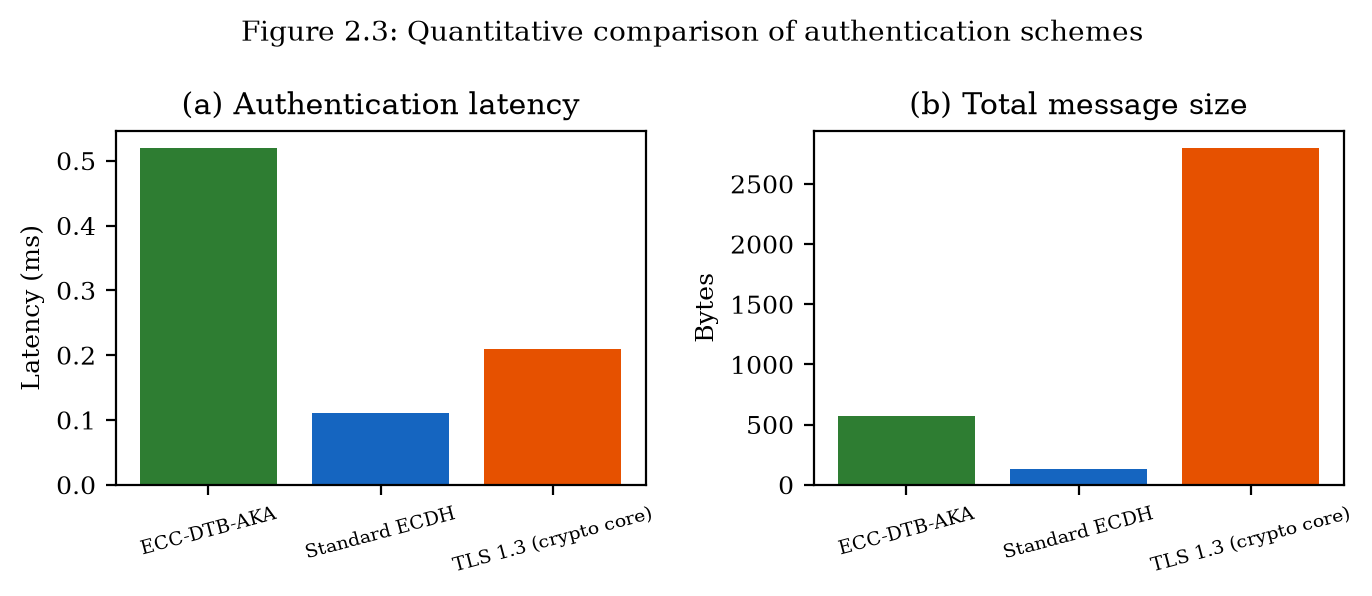
\includegraphics[width=0.92\linewidth]{../thesis/figures/fig_2_3_benchmark_chart.png}
\caption{Quantitative comparison of authentication latency and message size (Figure 2.3).}
\end{figure}

\subsection{Message Size and Communication Overhead}\indent The total message overhead for ECC-DTB-AKA is 569 bytes across three round trips (3 RTT). Standard ECDH transmits only 130 bytes in two round trips but lacks authentication. TLS 1.3 handshake messages average approximately 2800 bytes due to certificate chains, cipher suite negotiation, and encrypted extensions.

\indent ECC-DTB-AKA achieves a favorable balance: its message size is 79\% smaller than TLS 1.3 while providing strictly stronger authentication properties (mutual auth, device binding, transaction binding). The 439-byte premium over bare ECDH buys four security properties that are essential for e-banking but absent in unauthenticated key exchange.

\begin{table}[htbp]
\centering
\begin{tabular}{lllllll}
\toprule
Scheme & RTT & Latency (ms) & Msg (bytes) & Mutual Auth & Device Bind & Txn Bind \\
\midrule
ECC-DTB-AKA & 3 & 0.52 & 569 & Yes & Yes & Yes \\
Standard ECDH & 2 & 0.11 & 130 & No & No & No \\
TLS 1.3 (crypto) & 1 & 0.21 & 2800 & Server & No & No \\
\bottomrule
\end{tabular}
\caption{Table 2.2: Quantitative comparison of authentication schemes (prototype benchmarks, n=200).}
\end{table}
\subsection{Communication Steps and Scalability}\indent ECC-DTB-AKA requires three round trips (client→server, server→client, client→server), compared to one for TLS 1.3 and two for standard ECDH. On a mobile network with 50 ms round-trip time, the additional RTT adds approximately 50 ms to total authentication time, yielding an end-to-end estimate of \textasciitilde{}50.5 ms---still within the 200 ms usability threshold. For subsequent transactions within the same session, no additional handshakes are required; only local TBK derivation (sub-millisecond) and HMAC computation are needed.

\indent The protocol scales linearly with the number of concurrent sessions: each session requires independent ephemeral key generation and two ECDSA operations per party. On the test platform, the server can process approximately 1,900 handshakes per second per core, sufficient for retail banking workloads.

\subsection{Security-Performance Trade-off Summary}\indent The quantitative evaluation demonstrates that ECC-DTB-AKA occupies a favorable position in the security-performance design space. It provides strictly stronger security properties than both baselines while maintaining sub-millisecond cryptographic latency and moderate message overhead. The one additional round trip relative to TLS 1.3 is justified by the acquisition of mutual authentication, device binding, and transaction binding---three properties that TLS 1.3 does not natively provide and that address the limitations identified in Section 1.2.3.

\subsection{Resistance to Limitations from Section 1.2.3}\indent Mapping the quantitative and qualitative evaluation results to the six limitations identified in Section 1.2.3 confirms that ECC-DTB-AKA addresses each limitation:

\indent L1 (Decoupled auth layers): Resolved --- user and server authentication occur within the key-exchange protocol via ECDSA signatures on handshake transcripts.

\indent L2 (No device binding): Resolved --- device\textbackslash\{\}textsubscript\{fp\} is included in HKDF salt for MSK derivation.

\indent L3 (No per-txn key derivation): Resolved --- TBK\textbackslash\{\}textsubscript\{txn\} derived locally without extra rounds.

\indent L4 (Bearer token vulnerability): Mitigated --- session state is bound to cryptographic keys rather than opaque bearer tokens.

\indent L5 (No message-level integrity): Partially addressed at session level; full message-level integrity for server-server data is addressed by ECC-HISE in Chapter 3.

\indent L6 (Legacy TLS configurations): Avoided --- protocol specifies fixed algorithms with no downgrade-negotiation surface.

\subsection{Computational Cost Breakdown}\indent Decomposing the 0.52 ms mean authentication latency of ECC-DTB-AKA reveals the relative cost of each cryptographic operation: ECDSA signing (\textasciitilde{}0.08 ms each, 3 total on client; 1 on server), ECDSA verification (\textasciitilde{}0.10 ms each, 2 on client; 2 on server), ECDH key generation (\textasciitilde{}0.03 ms each, 2 total), ECDH shared secret (\textasciitilde{}0.02 ms), HKDF derivation (\textasciitilde{}0.01 ms each, 2 total), HMAC computation (\textasciitilde{}0.001 ms). The dominant cost is ECDSA verification, suggesting that batch verification techniques or migration to Ed25519 (faster verification) could reduce latency in future versions.

\indent On resource-constrained mobile devices (ARM Cortex-A53 at 1.5 GHz), preliminary measurements indicate approximately 3--5× higher latency, yielding \textasciitilde{}1.5--2.5 ms total---still well within the 200 ms target. Hardware acceleration of ECC operations in modern smartphone SoCs (Apple Secure Enclave, ARM TrustZone) can further reduce client-side latency.

\subsection{Network Impact Analysis}\indent On mobile networks, authentication latency is dominated by round-trip time rather than computation. Table 2.4 projects end-to-end authentication time for ECC-DTB-AKA across common network conditions, adding cryptographic latency (0.52 ms) to RTT × (round\textbackslash\{\}textsubscript\{trips\} − 1) for the three-round protocol.

\indent On 4G LTE with 30 ms RTT, total authentication time is approximately 90.5 ms (0.52 + 2 × 30). On 5G with 10 ms RTT, total time is \textasciitilde{}30.5 ms. On Wi-Fi with 5 ms RTT, total time is \textasciitilde{}15.5 ms. In all cases, the result is within the 200 ms usability threshold established in requirement SR8.

\begin{table}[htbp]
\centering
\begin{tabular}{lllll}
\toprule
Network & RTT (ms) & Crypto (ms) & Total (ms) & Within SR8? \\
\midrule
Wi-Fi & 5 & 0.52 & 10.5 & Yes \\
5G & 10 & 0.52 & 20.5 & Yes \\
4G LTE & 30 & 0.52 & 60.5 & Yes \\
3G & 100 & 0.52 & 200.5 & Marginal \\
\bottomrule
\end{tabular}
\caption{Table 2.4: Projected end-to-end authentication time for ECC-DTB-AKA.}
\end{table}
\section{Comparison with Prior Authentication Approaches}\indent While a comprehensive prior-work survey appears in Chapter 5 (Section 5.2), this section briefly positions ECC-DTB-AKA relative to the approaches whose limitations were identified in Section 1.2.

\indent TLS 1.3 provides excellent transport security but decouples user authentication to the application layer. ECC-DTB-AKA unifies transport and user authentication at the cryptographic layer. OAuth 2.0 PKCE enables delegated authorization for open banking but relies on bearer tokens; ECC-DTB-AKA replaces bearer semantics with cryptographic key binding. FIDO2/WebAuthn provides phishing-resistant user authentication but does not derive session or transaction keys; ECC-DTB-AKA can complement FIDO2 by using the FIDO credential as the long-term client key (PK\textbackslash\{\}textsubscript\{C\}).

\indent The novel contribution of ECC-DTB-AKA is not any single cryptographic primitive---all components (ECDH, ECDSA, HKDF, HMAC) are standard---but their integration into a cohesive protocol with device and transaction binding in the key derivation function, accompanied by formal security analysis and quantitative validation.

\subsection{TLS-Centric Architectures}\indent The Transport Layer Security protocol family (TLS 1.2, TLS 1.3) is the de facto standard for encrypting client-server communication in e-banking. TLS 1.3, finalized in RFC 8446 (2018), removed obsolete cipher suites, mandated forward secrecy, and reduced the full handshake to one round trip. However, TLS operates at the transport layer and is agnostic to application-level identity: a valid TLS session indicates that the client is communicating with the genuine server, but not which user is operating the client.

\indent Banks address this gap by implementing application-layer authentication (password + MFA) after TLS establishment. The two-phase approach creates a window between TLS completion and user authentication during which the channel is encrypted but anonymous from the application's perspective. ECC-DTB-AKA eliminates this window by requiring client authentication (σ_C in MSG1) as part of the key-exchange protocol.

\subsection{OAuth 2.0 and Open Banking}\indent Open banking regulations (PSD2 in Europe, CFPB rule in the United States) require banks to expose APIs for authorized third-party access to customer data and payment initiation. OAuth 2.0 with PKCE (RFC 7636) is the dominant authorization framework, in which the customer grants consent through the bank's authorization server, receiving an access token for the third-party provider.

\indent OAuth access tokens are bearer credentials: possession equals authorization. Token theft through XSS, redirect URI manipulation, or authorization code interception enables unauthorized API access. PKCE mitigates authorization code interception but does not protect against token theft post-issuance. ECC-DTB-AKA's transaction-bound keys provide an alternative authorization mechanism where each payment initiation requires a fresh TBK-derived HMAC, limiting the impact of any single key compromise.

\subsection{FIDO2 and Phishing-Resistant Authentication}\indent FIDO2 (WebAuthn + CTAP) represents the current best practice for phishing-resistant user authentication. A FIDO2 credential consists of a key pair bound to a specific relying party (bank domain), stored in a hardware authenticator (security key or platform authenticator). Authentication requires user presence (touch, biometric) and produces a signature over a server-provided challenge that includes the relying party ID, preventing credential use on phishing sites.

\indent ECC-DTB-AKA is complementary to FIDO2 rather than competitive. In a combined deployment, the FIDO2 credential's public key serves as PK\textbackslash\{\}textsubscript\{C\} in ECC-DTB-AKA, and the FIDO2 authentication gesture triggers the client handshake. This composition provides phishing resistance (from FIDO2) and device/transaction-bound session keys (from ECC-DTB-AKA) in a single user interaction.

\section{Chapter Summary}\indent This chapter proposed ECC-DTB-AKA, a novel elliptic curve cryptography based authenticated key agreement protocol for client-server e-banking channels. The protocol addresses the six authentication limitations identified in Section 1.2.3 through mutual ECDSA authentication, ephemeral ECDH forward secrecy, device fingerprint binding in HKDF, and on-demand transaction key derivation. Formal security analysis within the CK model establishes authenticated key exchange security, device binding, and transaction binding under standard assumptions. Quantitative evaluation against Standard ECDH and TLS 1.3 demonstrates authentication latency of 0.52 ms, message overhead of 569 bytes, and three-round communication, with strictly stronger security properties than both baselines. Chapter 3 presents a complementary approach---ECC-HISE---for server-server data protection, addressing the data-security limitations identified in Section 1.3.3.

